Модель Transformer является архитектурой глубокого обучения, предназначенной для
обработки последовательных данных,
таких как тексты или временные ряды.
Она была предложена в статье \cite{vaswani2017attention} 
и стала одной из самых инновационных архитектур
в области обработки естественного языка.

Основной компонент модели Transformer это механизм внимания. Он позволяет модели сосредоточиться 
на наиболее важных частях входных данных при выполнении задач, таких как машинный перевод или обработка текста.

\begin{figure}[h]
    \centering
    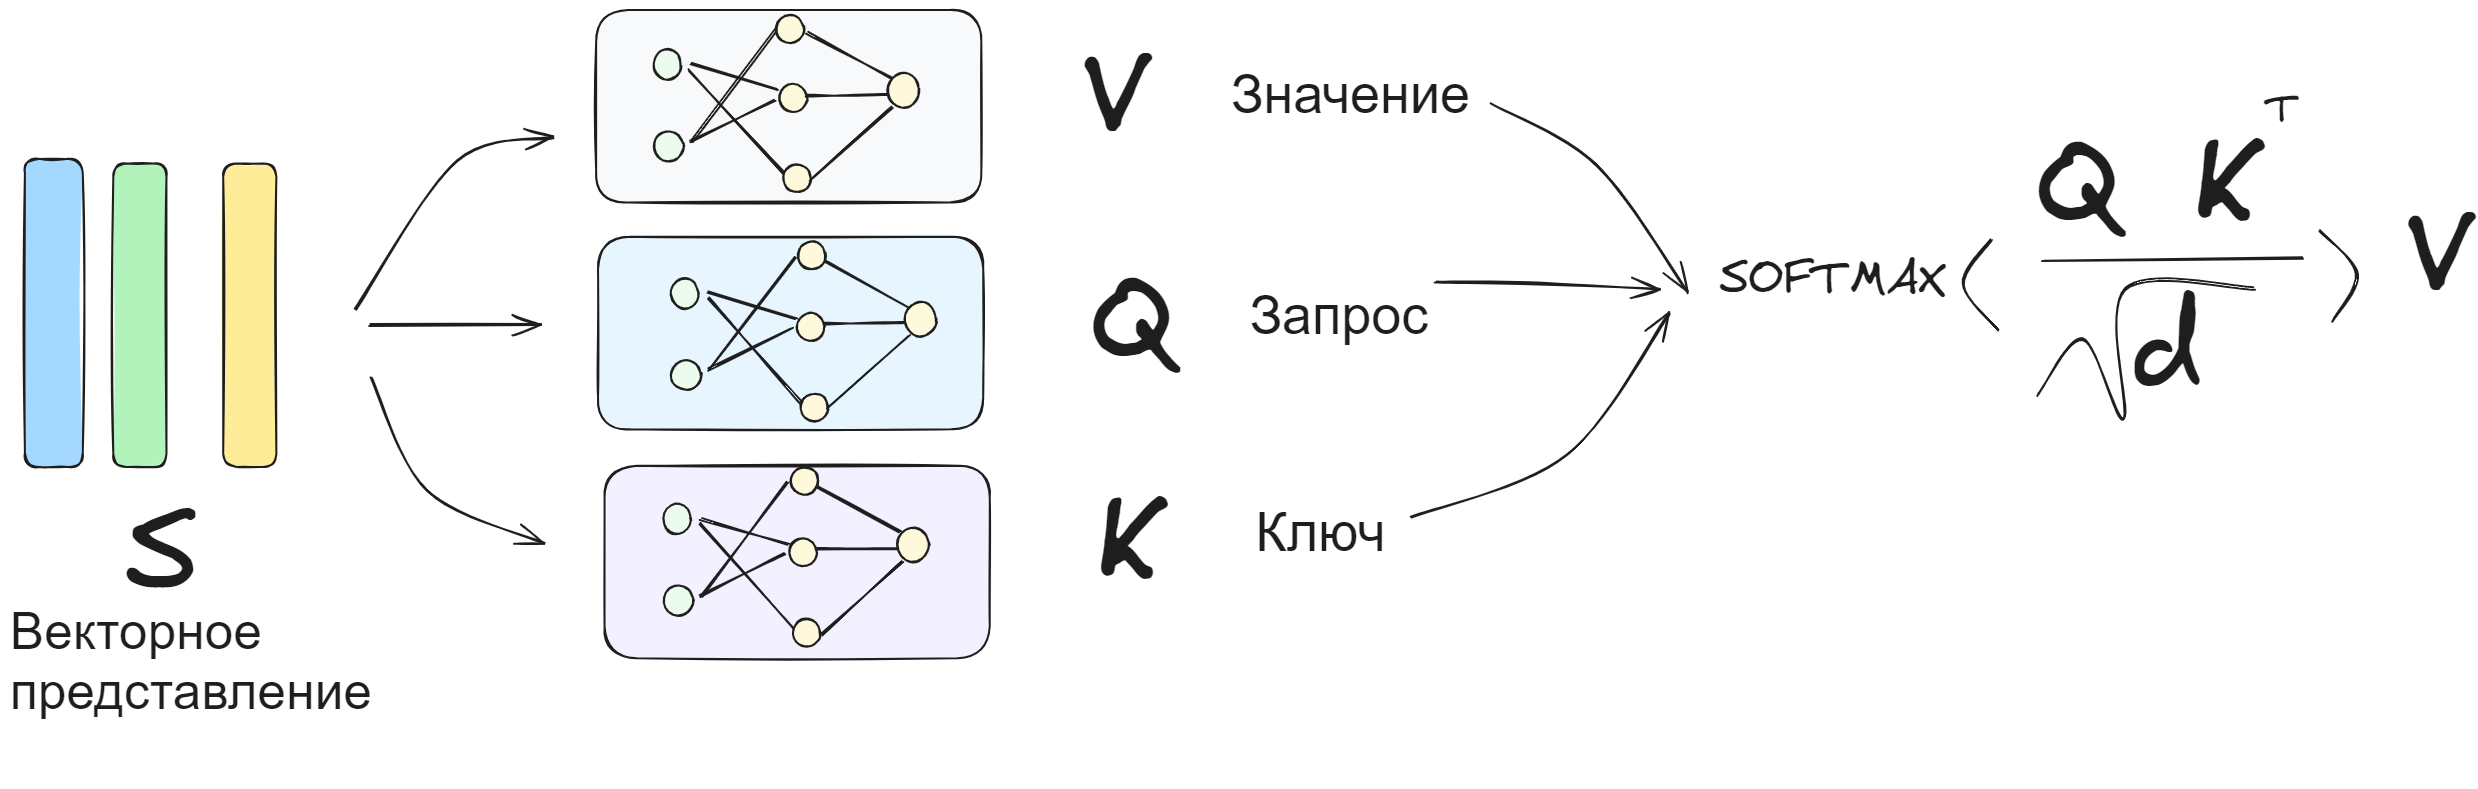
\includegraphics[width=0.5\textwidth]{assets/ml/nn/transformer.excalidraw.png}
    \caption{Механизм внимания в архитектуре Transformer (Self Attention) \cite{vaswani2017attention} }
    \label{self_attention}
\end{figure}

Подробнее опишем механизм внимания.
Механизм внимания в Transformer состоит из трех основных частей:\begin{enumerate}
    \item  расчета векторов запроса, ключа и значения.
    Они используются для вычисления весов входных данных и определения их важности для каждого элемента:
    \begin{equation}
        \begin{aligned}
            &q =W_q x \\ 
            &k = W_k x \\
            &v = W_v x,
        \end{aligned}
    \end{equation}
    где \(W_q\), \(W_k\), \(W_v\) - матрицы весов, которые модель обучает.
    \item вычисления векторов запроса и ключа, для каждого элемента \(x_i\) вычисляются логиты \(e_{ij}\):
    \begin{equation}
        e_{ij} = \frac{q \cdot k_j}{\sqrt{d_k}} ,
    \end{equation}
    где \(d_k\) - длина запроса,
    \item преобразуются в веса внимания \( \alpha_{ij} \) с помощью функции softmax:
    \begin{equation}
        \alpha_{ij} = \frac{\exp(e_{ij})}{\sum_{j'} \exp(e_{ij'})}.
    \end{equation}
\end{enumerate}

Эти веса показывают, какую важность модель придает каждому элементу данных при решении конкретной задачи. 
После вычисления весов внимания, они умножаются на соответствующие значения (value) и суммируются, чтобы получить итоговый взвешенный вектор, который представляет собой выход механизма внимания.